\section{\sysname Architecture} \label{sec:hardenUI}
% Protecting User Input Integrity by Visual Supervision}

 Now we describe how \sysname addresses the challenges (refer to. Section~\ref{sec:systemDesign:challenger}) to ensure that all remote requests truly correspond to a legitimate user's intended input. \sysname has two major components: \name server-side component and \name phone app. \name server-side component instruments the webpage with visual cues that help the \name application for the image processing of the web page. The server-side component also sends a signed specification of the given form to the phone app. This specification serves as the ground truth. \name phone app processes the rendered form on the client's screen and detects any changes as per the form specification. Additionally, it also records all the user inputs. The \name server-side component receives input data from both the browser and the phone app and checks for discrepancies. In the following, we discuss these two components in details and show how we address the challenges. We assume a typical PKI scenario where the phone app knows the public key of the server. The phone app also generates a keypair and signs the data submitted to the server. We also assume there is an offline registration phase by which the server learns the \sysname application's public key.

\begin{figure}[t]
	\centering
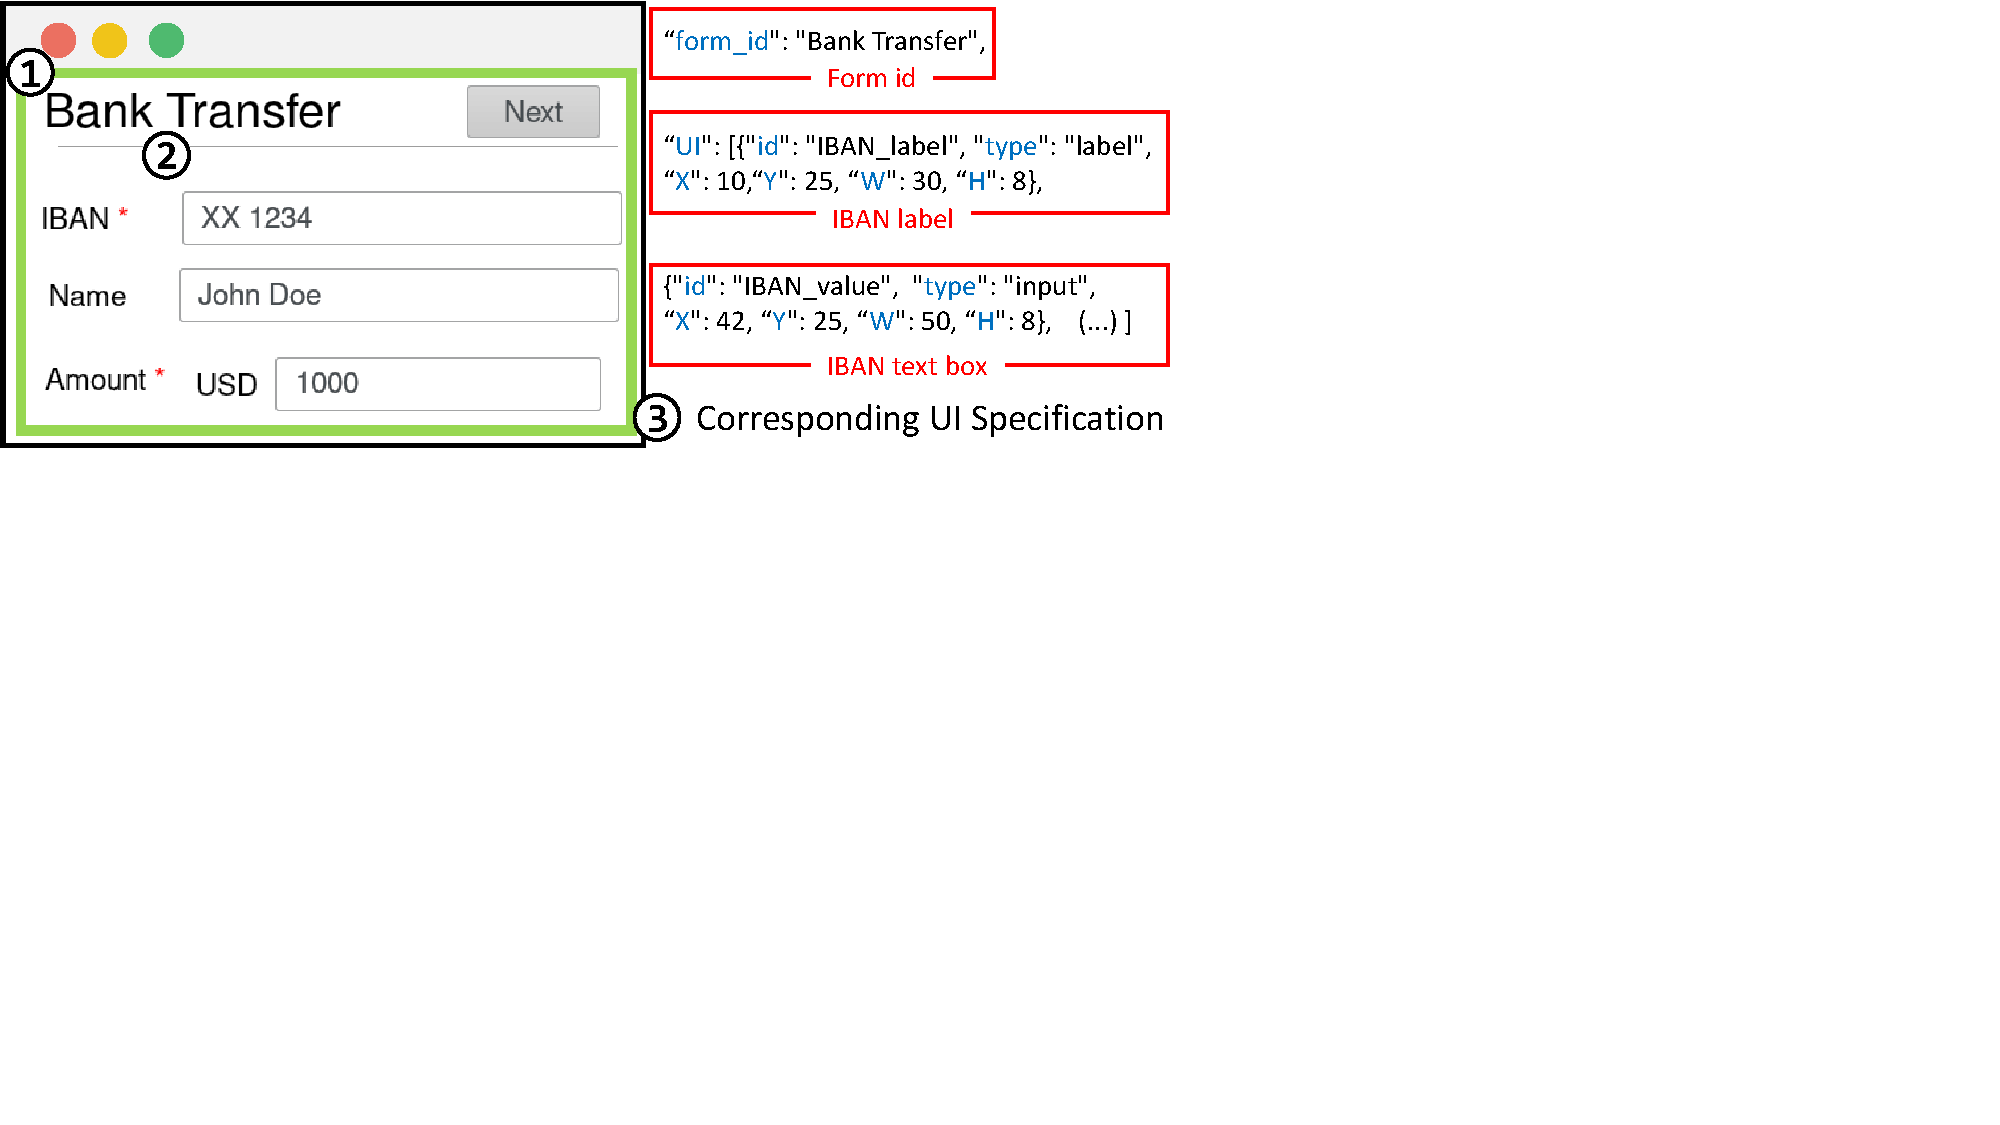
\includegraphics[trim={0 11.5cm 14cm 0},clip, width=0.8\linewidth]{chapters/IntegriScreen/newImg/runningExample.pdf} 
	\caption[Example web form and specification generated by the \name server-side component]{Example web form and specification generated by the \name server-side component.}
	\label{fig:runningExample}
\end{figure}



\subsection{Server-side Component}
\label{sec:systemDesign:webserver}

\name server-side component is responsible for: i) instrumentation of the web form, and ii) input trace matching. We use the web form depicted in Figure~\ref{fig:runningExample} as a running example.

\subsubsection{Instrumentation of the web form}
\label{sec:systemDesign:webserver:instr}

\name server-side component carries out the following instrumentation in the web form as depicted in Figure~\ref{fig:runningExample}:

\begin{enumerate}	

\item[\one] \emph{Form Border} \sysname server-side component puts a visible boundary around the UI that aids the \sysname phone app to detect the form and align it properly. For simplicity, the current prototype uses a solid green color to indicate the form border.
However, this can be fully customized as long as the four corners that indicate the protected area can be detected and tracked by the mobile app~\cite{zhang2002visual}.



\item[\two] \emph{Form Title} The title serves as a unique identifier corresponding to a UI form and its corresponding specification.

\item[\three] \emph{Form Specification} The \sysname phone app receives a form specification from the server-side component signed by the server. This specification dictates the type and location of UI elements relative to the form boundary (refer to the example specification in Figure~\ref{fig:runningExample}). This specification serves as ground truth for the phone app to verify the UI integrity on the client's screen. The specification can either be provided by developers of the remote service or automatically generated by the \sysname server component.

\end{enumerate}

\subsubsection{Input trace matching}

\sysname requires a server-side component that carries out the \emph{input trace matching} between: i) the user input from the HTTP payload sent by the browser, and ii) signed input from the \sysname \tls payload. One such example is illustrated in Figure~\ref{integriscreen:fig:systemModel}. If these two traces mismatch, the \name server-side component notifies the \name phone app.



\begin{figure}[t]
	\captionsetup[subfigure]{justification=centering}
	\centering
	\null
	\hfill
	\subfloat[App verifies all UI elements, instructs users to input data.] 
	{
		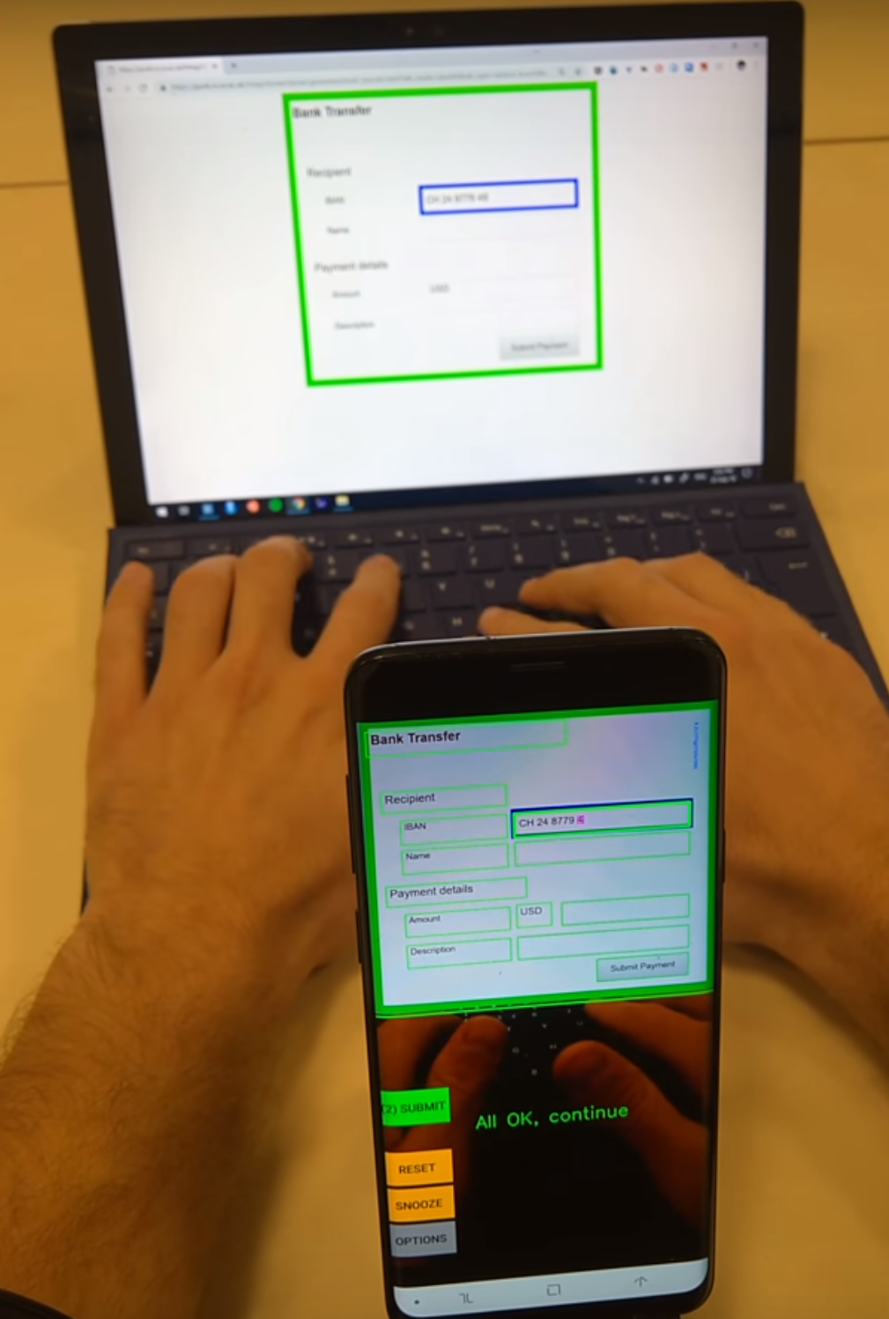
\includegraphics[width=0.4\columnwidth]{chapters/IntegriScreen/img/IntegriscreenAllOK_cropped.PNG}
		\label{fig:userExperience:UIVerificationSuccess}
	}
	\hfill
	\subfloat[Server comparison mismatch shown on the smartphone.] 
	{
		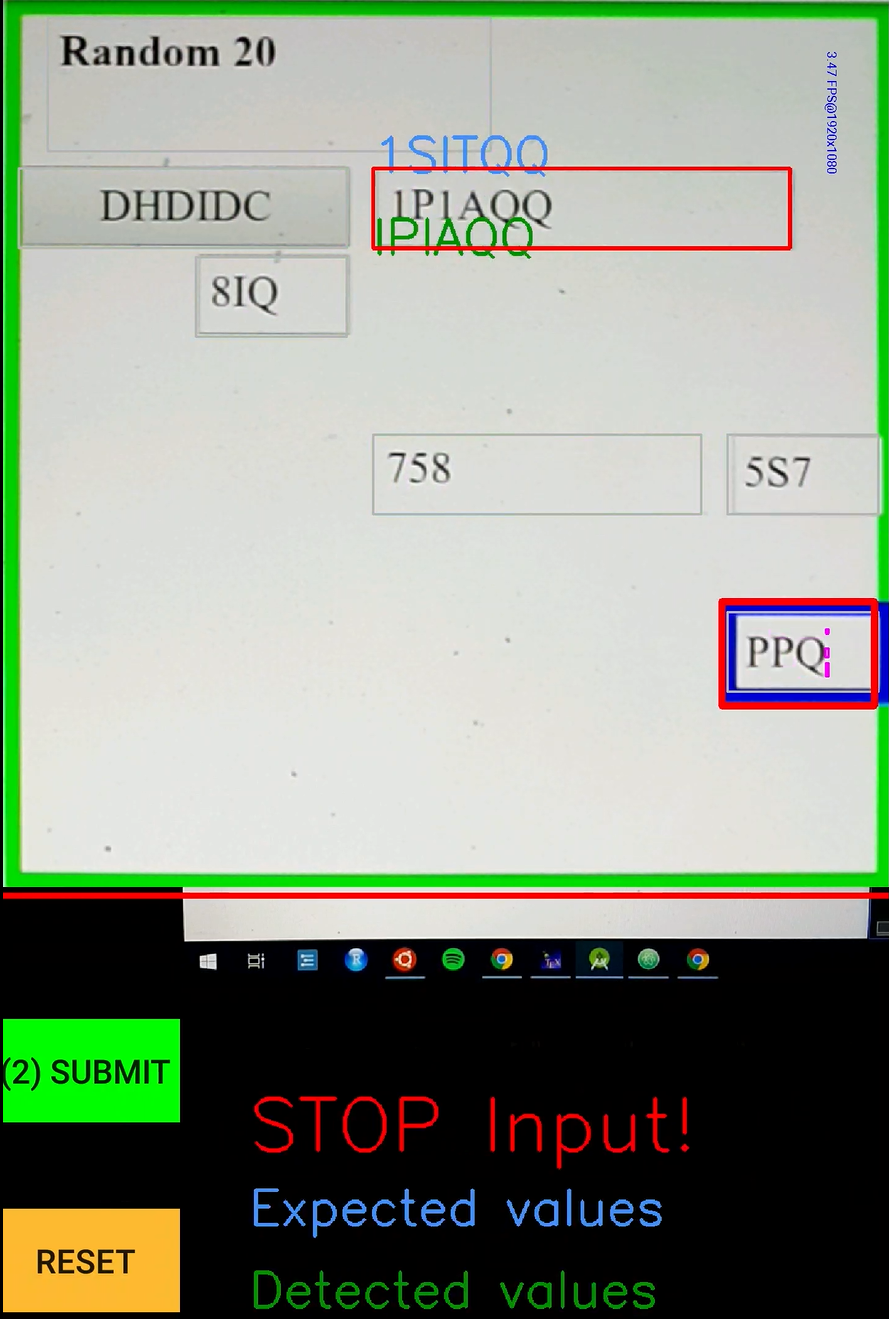
\includegraphics[width=0.4\columnwidth]	{chapters/IntegriScreen/img/DetectingChanges_cropped.PNG}
		\label{fig:userExperience:inputSupervision}
	}
	\hfill
	\null
	\caption{
		User experience of the smartphone app.
}
	\label{fig:userExperience}
\end{figure}




\subsection{\sysname Application} 
\label{sec:systemDesign:phone}

The app provides a second-factor confirmation of user's intended input. This is achieved by verifying that the user interface matches its specification during user interaction, supervising against any on-screen modification attacks, and capturing the data shown on the screen to generate and send a respective \POI. After the user starts \sysname app, it performs the following steps:

\begin{enumerate}
    \item \emph{Locates} the border of the web form on the client's display, realigns the captured video feed to a flat perspective (as shown in Figure~\ref{fig:userExperience:UIVerificationSuccess}), and extracts the form's unique title.
    \item \emph{Loads} the corresponding UI specification file sent by the server. The app verifies the signature.
    \item \emph{Continuously verifies that the UI} of the web form shown on the client device matches its specification, i.e., that all UI elements are present and that none have been modified or added.
    \item \emph{Continuously supervises user input}, allowing only the element in focus to change, only when the user is present and active.
	\item \emph{Submits} the generated \POI to the server. Note that this data is signed and replay protected with a nonce.
    \item \emph{Notifies} the user about the result of server's data comparison: either success (if client and \md -submitted data match) or failure (in case of data mismatch). In the latter case, the user can choose one of two versions of submitted data (or a combination thereof). For additional security guarantees, the user confirms her choice in a hardware protected user interface which is available since Android 9~\cite{androidConfirmation}.
\end{enumerate}

We will now expand on steps \emph{(3)} and \emph{(4)}: the core of the \name mobile app, as they are continuously executed for each frame that the app captures to protect IO integrity.


\subsubsection{Continuous UI Verification}
\label{sec:systemDesign:phone:uiVerification}
Initially the app downloads the UI specification from the server and validates its signature. Afterwards it checks if the UI elements captured by the camera \textit{comply} to the specification. The form name is an unique identifier (refer to Section~\ref{sec:systemDesign:webserver:instr}) that ensures that the phone app uses the appropriate specification for the form shown on the client's screen. In the case of a mismatch, the application warns the user of a potential attack, both visually and by ringing or vibrating. The application clearly augments its preview of the screen (refer to Figure~\ref{fig:userExperience:inputSupervision}) to show which elements are problematic (showing them in red), and prevents any data input until the mismatch is corrected.

\subsubsection{Continuous Input Supervision}
\label{sec:systemDesign:phone:inputerSupervision}

Besides the layout of the UI, the app supervises continuously UI changes on the form to make sure it is a result of intended user interaction:

\myparagraph{Only the element in focus can change} \name app can detect which UI element is in focus. The app mandates that except the element in focus, all other elements must remain the same. This ensures that the user needs to only pay attention to the value of the currently active element (which they are editing), while all other elements are \emph{protected}.

\myparagraph{Activity detection} If the value of the active element changes, the app also ensures that the user is present by detecting user's hands from the camera feed.

\myparagraph{Focus cool-down time} If the value of some active element changes, the focus should not change to another element in less than $x$~ms after the last edit and in less than $y$~ms since this element first came into focus. The server can optionally set the values of $x$ and $y$ in the specification file. In our prototype, we set $x=300$~ms and $y=2$~s. This mechanism serves two goals: (i) ensures that any change can be correctly detected, given frame rate limitations of the mobile app; and (ii) ensures that the adversary can not quickly move the focus to another element and change its value without the user noticing. We experimentally evaluate these assumptions in Section~\ref{sec:experimentalEvaluation} and show an example of input supervision detecting malicious modification in Figure~\ref{fig:userExperience:inputSupervision}.

\myparagraph{Supervised form submission} Furthermore, to prevent the adversary from prematurely submitting the form, the \POI is submitted to the server only after the user explicitly presses the \emph{Submit} button on the mobile device.


\myparagraph{Occlusion and multi-page forms}
Our system design supports user interactions in which the form is temporarily occluded (e.g., changing browser tab, minimizing the browser window).
In such cases, UI verification temporarily fails, but will be resumed as soon as the form is displayed again on the client's screen: if the values of all elements are unchanged, user input is allowed again. Such a design also supports multi-page interfaces, as the application will simply store the values of all input elements on each page as the user edits them in arbitrary order. Changes to hidden elements are rejected, and the value is verified every time the element is displayed again.